\documentclass[12pt,letterpaper]{article}
\usepackage[utf8]{inputenc}
\usepackage[english]{babel}
\usepackage{listings}
\usepackage{xcolor}
\usepackage{graphicx}

%For syntax highlighting
\definecolor{codegreen}{rgb}{0,0.6,0}
\definecolor{codegray}{rgb}{0.5,0.5,0.5}
\definecolor{codepurple}{rgb}{0.58,0,0.82}
\definecolor{backcolour}{rgb}{1,1,1}

%%Sets different parameters
\lstdefinestyle{mystyle}{
	backgroundcolor=\color{backcolour},   
    commentstyle=\color{codegreen},
    keywordstyle=\color{magenta},
    numberstyle=\tiny\color{codegray},
    stringstyle=\color{codepurple},
    basicstyle=\ttfamily\footnotesize,
    breakatwhitespace=false,         
    breaklines=true,                 
    captionpos=b,                    
    keepspaces=true,                 
    numbers=left,                    
    numbersep=5pt,                  
    showspaces=false,                
    showstringspaces=false,
    showtabs=false,                  
    tabsize=4
}
\lstset{style=mystyle}

\title{\textbf{Department of Computer Science and Engineering}}
\author{\textbf{S.G.Shivanirudh , 185001146, Semester VI }}

\date{14 April 2021}

\begin{document}
\maketitle
\hrule
\section*{\center{UCS1601 - Internet Programming}}
\hrule 
\bigskip\bigskip

%Assignment name
\subsection*{\center{\textbf{Assignment 6:  Autocomplete Feature using AJAX}}}

%Objective
\subsection*{\flushleft{Objective:}}
\begin{flushleft}
    Develop  an  AJAX  program  that  implements  the  Autocomplete  feature  for  filling the country names as given.
\end{flushleft}

%Code
\subsection*{\flushleft{Code:}}
\subsubsection*{\flushleft{HTML:}}
\begin{flushleft}
\lstinputlisting[language = HTML]{index.html}
\end{flushleft}

\subsubsection*{\flushleft{CSS:}}
\begin{flushleft}
\lstinputlisting{styles_index.css}
\end{flushleft}

\subsubsection*{\flushleft{Country Servlet:}}
\subsubsection*{\flushleft{Java:}}
\begin{flushleft}
\lstinputlisting[language=Java]{Country.java}
\end{flushleft}

\subsubsection*{\flushleft{XML:}}
\begin{flushleft}
\lstinputlisting[language=XML]{WEB-INF/web.xml}
\end{flushleft}

\newpage
%Output
\subsection*{\flushleft{Output:}}
\subsubsection*{\flushleft{Initial:}}
\begin{figure}[h]
    \centering
    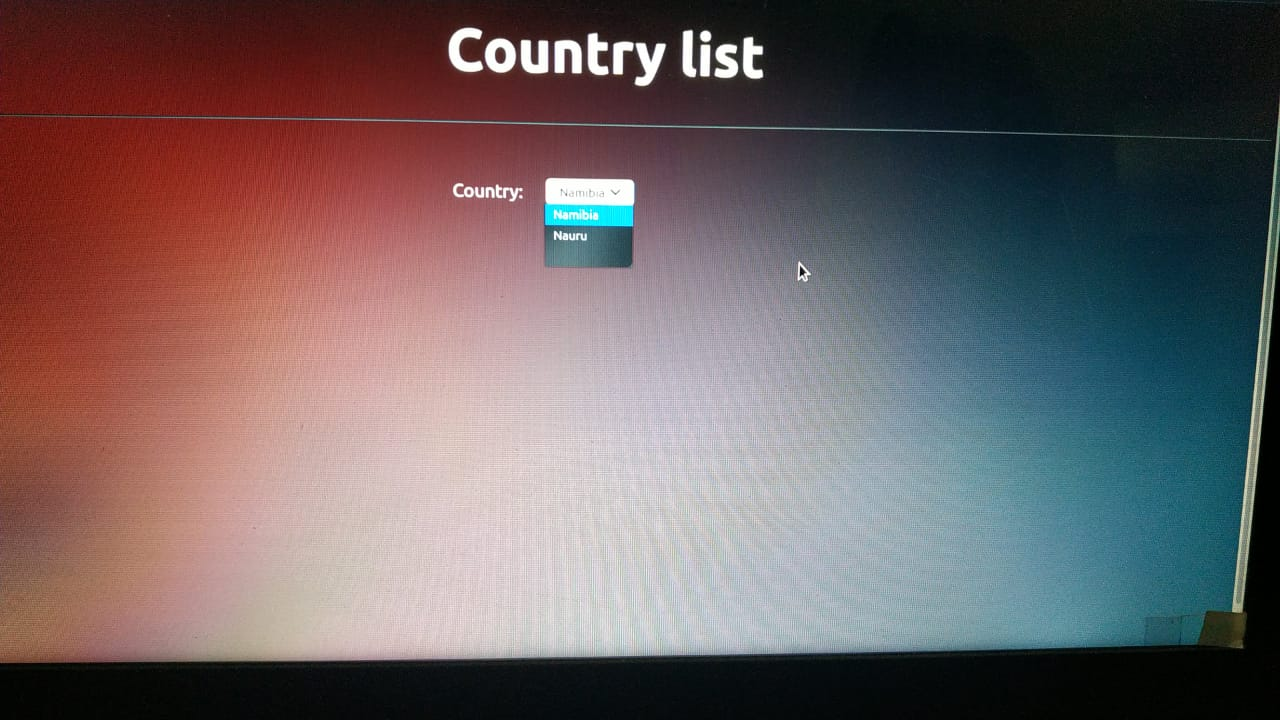
\includegraphics[width = \textwidth]{Pics/op1.jpeg}
\end{figure}
\newpage
\subsubsection*{\flushleft{Input "n":}}
\begin{figure}[h!]
    \centering
    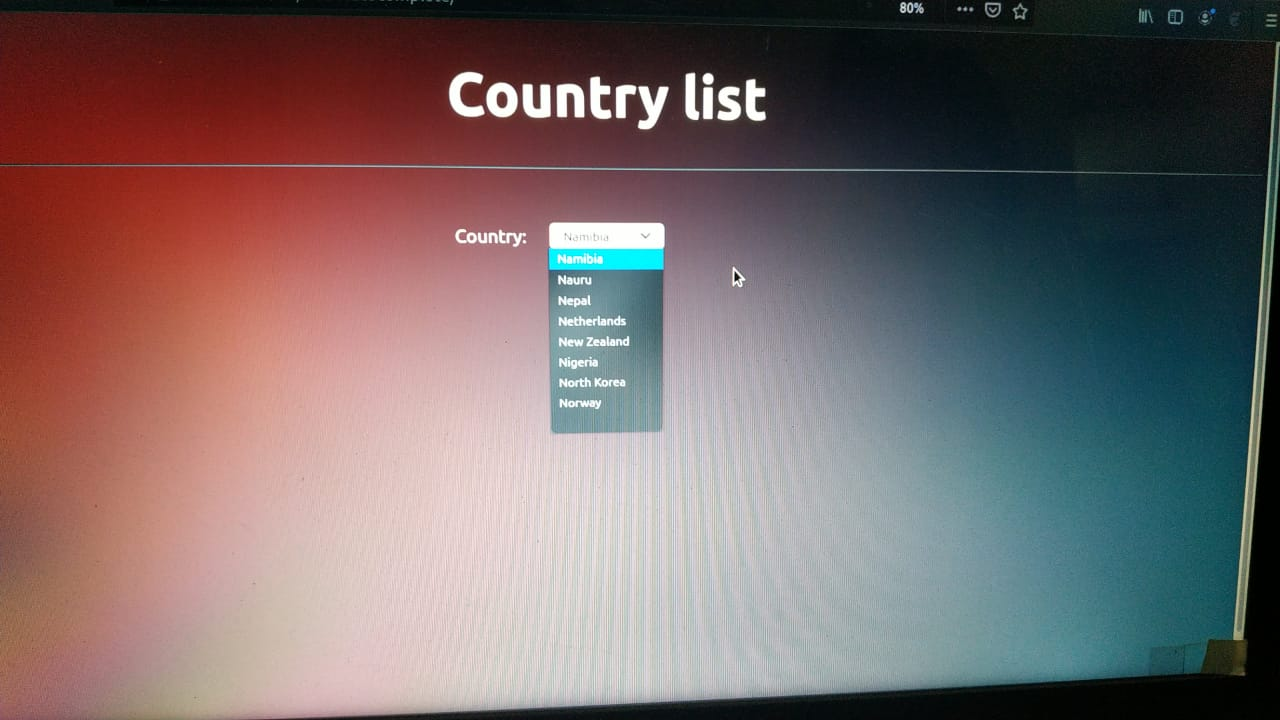
\includegraphics[width = \textwidth]{Pics/op2.jpeg}
\end{figure}
\newpage
\subsubsection*{\flushleft{Input "na":}}
\begin{figure}[h!]
    \centering
    
\includegraphics[width = \textwidth]{Pics/op3.jpeg}
\end{figure}

\hrule
\end{document}